\documentclass[a4paper,11pt]{article}

\usepackage[latin1]{inputenc}
\usepackage[english]{babel}
\usepackage{graphicx}
\usepackage[a4paper,top=2cm,bottom=2cm,left=3cm,right=3cm]{geometry}
\graphicspath{ {./} }
%\graphicspath{ {./images/} }

\usepackage{listings}
 


\title{Binary Tree}
\author{Davide Scassola, Salvatore Milite}


\begin{document}
\maketitle

The aim of the project is to implement a Binary Tree in c++ and compare its performance with std::map. The work is organized in three directories: in the \emph{include} directory there is the templated class, in the \emph{test} one there is the unit test and the generated documentation is in \emph{documentation}. There is also an \emph{old} with an early iterative version of the code. The benchmarks where we compare our version of the data structure against std::map and where we test our balance algorithm is in the main folder.  


\section*{Code and implementation}

The BinaryTree class is templated with three arguments, the key type, the value type and the function used for comparison, in particular the default is std::less$<$value\_type(key)$>$, a functional object that returns, when it is called with its two arguments, \emph{arg1 $<$ arg2}. The class has a unique\_pointer to the root node and an instance of the comparison callable object. Throughout the code we decided to use smart pointers to make easier the memory management and to avoid to write a custom destructor.  

\subsection*{Node class}

The node data structure is nested into the class, we opted for this choice in order to preserve a coherence between the templates as well as a logical dependency(indeed we do not have to instantiate node objects outside of the class). The Node object is constructed with those attributes 

\begin{itemize}
\item a unique\_pointer to the right node

\item a unique\_pointer to the left node

\item a pointer to the parent (this pointer does not have to release memory)

\item a std::pair with const key and value
\end{itemize}

\subsection*{Iterators}

The class is equipped with two types of iterators: const and non const, defined as internal classes with a pointer to a node. The iterators have overloaded the operators: $*$(), which returns a std::pair$<>$ from the node; $++$(), which returns an iterator to the next node (next with respect to the order of the keys) and $++$(int) with the usual behavior. 

\subsection*{Methods}

The BinaryTree class has implemented the copy behavior (it creates a deep copy of tree with a recursive algorithm) and the move semantic; it also has a default constructor which initializes a void tree or can take the functional object as an argument (the destructor is the default). Regarding the other method we tried to make code as simple as possible, so we did a wide use of recursion, and most of the algorithms are recursive. The functions insert() and find() use a common private method named search() which returns, given a key and a pair of node pointers, a reference to the node that matches the key or to the node corresponding to the insert position of that key. Actually, search returns a std::pair with a reference to a node pointer(the one described before) and a pointer, the latter is the pointer to the parent. This choice has been made as to remove some if statements(the root can be treated as an ordinal node) and make easier to assign the parent node. Indeed, when we assign the parent, if the node is on the right, we consider as its parent its parent's parent(i.e. the first greater parent). In these way the $++$() operator is easier to implement. The insert() method can work in two scenarios: 
\begin{itemize}
	\item the key is not present; in this case the function inserts the node and returns an std::pair with an iterator to the new node and a \emph{bool} with the value true
	\item the key is present; in this case the function returns an std::pari consisting of an iterator to the node with the same key used for the search and a \emph{bool} with the value false. Is up to the user the final choice of changing the value inside.
\end{itemize}

The balance() function is recursive. It first transforms the tree into a vector of std::pairs and after it  constructs the balanced tree splitting the list and inserting the node in its middle. It after calls balance(std::vector<std::pair> list, Iterator begin, Iterator end) on the halves recursively, till there are no more nodes to insert.
The const operator[] return a std::runtime\_exception if a non valid key is accessed.
There are also some test methods which are defined and declared only when loaded in the unit test that find the height of the tree and weather it is balanced or not. 
The unit test makes use of the catch2 unit testing framework, which is a collection of macros stored in the \emph{catch.hpp} file and speeds up the writing of the test code. 

\section*{Performance measures}
In order to evaluate the performances of our implementation of the binary tree, we ran some tests.
The test involves four different types of tree: a "linked-list" tree, created inserting elements orderly (with respect to the key), a random tree, created inserting elements wich keys were in random order, a balanced tree, created copying and balancing the random tree, and finally the std::map.

The benchmark consists (for each tree) in accessing all the elements and measuring the average access time:
In the case of the linked-list-tree we expect to see a time that is $O(n)$ with respect to the tree size, for the balanced and the std::map we expect to see $O(\log_2 n)$. 
The results are shown in microseconds, and code is compiled with the level O3 of optimisation.\\

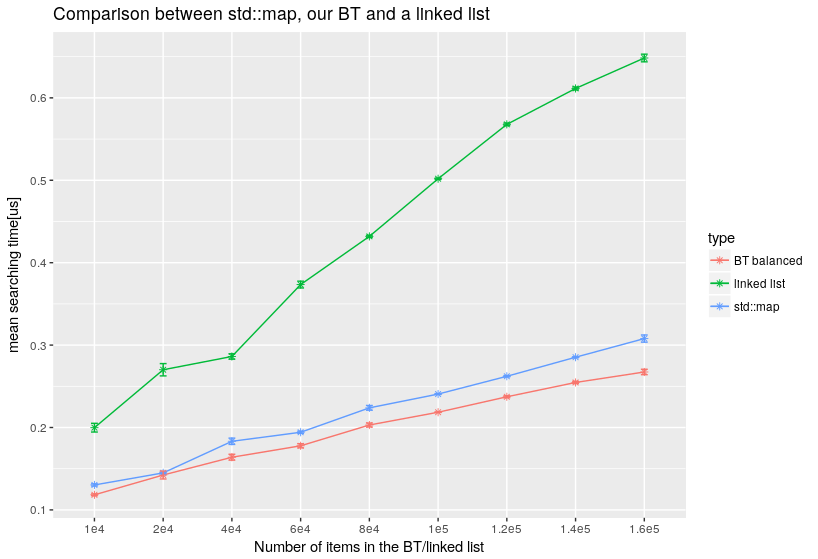
\includegraphics[height=10cm]{./LL_vs_BT.png}\\

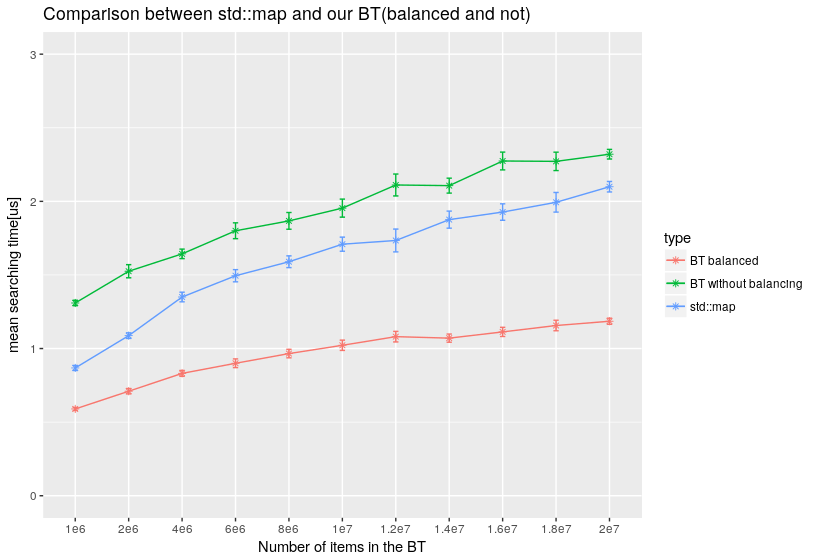
\includegraphics[height=10cm]{./map_vs_BT.png}\\

From the plots it seems that the previous considerations about the time complexity hold.
We can see that even though balancing the tree improves dramatically the performances with respect to the linked list tree (about 1000 times), also the not perfectly balanced random tree is quite good and in this case the speedup is less than 2.

Surprisingly we performed better than the std::map, our guess is that our simple code is easier to optimize for the compiler, and maybe the std::map spends time in checks and other procedures we don't know.
However, we verified that with the lowest level of optimization (O0), the stp::map runs faster.


\vspace{2cm}

\end{document}